\documentclass[a4paper,10.5pt,uplatex]{jsarticle}  %jsarticleでも良いかも
%--脚注の設定
\usepackage{natbib}
\bibpunct[, ]{(}{)}{;}{and}{}{,} %本文での引用の体裁はここで整えられるみたい
\bibliographystyle{apsr2006-2}   %このagsmは編集済みなので注意。ジャーナルが太字にならないようにしてる。ブログ参照。
\usepackage{amsmath}
%--余白の設定
\usepackage[truedimen,margin=20truemm]{geometry}
%--図の設定
\usepackage[dvipdfmx]{graphicx} % PDFの利用もOKに
\graphicspath{{./figures/}} %To add paths relative to the latexfile invoking the command
%--行間の設定
\usepackage{setspace} 
\setstretch{1.13} % ページ全体の行間を設定
%コードの設定
\usepackage{listings}
\usepackage{color}
\definecolor{dkgreen}{rgb}{0,0.6,0}
\definecolor{mygray}{rgb}{0.5,0.5,0.5}
\definecolor{mauve}{rgb}{0.58,0,0.82}

\definecolor{codegreen}{rgb}{0,0.6,0}
\definecolor{codegray}{rgb}{0.5,0.5,0.5}
\definecolor{codepurple}{rgb}{0.58,0,0.82}
\definecolor{backgroundcolour}{RGB}{247,247,247}

\lstset{ %
  language= {Python}, %ここを含めなければ、変に太字になったりしない
  aboveskip=2.5mm,
  belowskip=4.5mm,
  showstringspaces=false,
  columns=flexible,
  keepspaces=true,
  numbers=left,                    
  numbersep=5pt,    
  basicstyle={\small\ttfamily},
  commentstyle={\small\ttfamily},
  breaklines=true,
  breakatwhitespace=true,
  tabsize=3,
  frame=single,
  backgroundcolor=\color{backgroundcolour},   
  commentstyle=\color{codegreen},
  keywordstyle=\color{magenta},
  numberstyle=\tiny\color{codegray},
  stringstyle=\color{codepurple},
	xleftmargin = 1.1cm,
  framexleftmargin = 1em
}
\usepackage{xcolor}
\usepackage{framed}
\colorlet{shadecolor}{green!8}
%リンクの埋め込みを可能にする  \href{ **URL** }{表示テキスト}
\usepackage[dvipdfmx]{hyperref}
\usepackage{courier}
\usepackage{here}
%日本語環境用の設定を追加
\usepackage[english]{babel} % まとめて英語化できる
\addto\captionsenglish{\renewcommand{\figurename}{Figure }}
\addto\captionsenglish{\renewcommand{\tablename}{Table }}
\renewcommand{\lstlistingname}{Code}
\usepackage{multirow}
\usepackage{placeins}
%数学用のフォント
\usepackage{amsmath} 
\usepackage{amssymb}
\usepackage{amsfonts} 
%Table of Contents
\setcounter{tocdepth}{3}
%-----------------
\begin{document}
\title{Sampling Methods}
\author{@Shusei-E}
\date{\today}
\maketitle
\begin{abstract}
Various ways to draw samples from distributions that are analytically hard to compute.
\end{abstract}

\noindent\rule{17.5cm}{1.7pt}
\vspace{-1.3cm}
\tableofcontents
\noindent\rule{17.5cm}{1.7pt}

\textbf{\Large \textcolor{red}{Metropolis-Hastings codes are old version! Please refer to the Jupyter notebook on GitHub.}}

\section{Bayesian Method}
The most important thing is \begin{equation}P(\theta|D) \propto P(D|\theta) P(\theta).\label{Eq:Bayes}\end{equation} Suppose we want to do Bayesian linear regression.
\begin{align}
  P(y) = \mathcal{N}(a+bx, \sigma^2) P(a, b, \sigma^2)
\end{align}
If we only focus on the likelihood, we can think we used the uniform distribution as a non-informative prior (read \S\ref{Sec:MLEMCMC} for detail), but it is better to include prior distribution.


\subsection{Likelihood function}
A likelihood is the probability of getting the data (observations) under certain parameters (あるパラメータにおいてその観測値が得られる確率), which means it is a function of prior distribution.\par
Suppose we have a random variable $Y \sim p(y|\theta)$. If we get $n$ independent observations, a joint probability of these observations is $$p(y|\theta) = \prod_{i=1}^{n} p(y_i | \theta).$$ If we set the prior distribution $p(\theta)$, the probability of getting the observations under the distribution $p(\theta)$ is $$p(y|\theta)p(\theta).$$Likelihood can be defined as $$L(\theta|y) = \prod_{i=1}^{n} p(y_i|\theta).$$ We use maximum likelihood estimation to search the parameters that can maximize the likelihood.

\subsection{MLE and MCMC}\label{Sec:MLEMCMC}
We can use MCMC instead of MLE to find the parameter (parameter's distribution). MCMC samples from the probability distribution that is proportional to the likelihood. To be precise, a statistical model can define a likelihood under the data you have. MCMC can get random samples from the parameter's distribution that is proportional to the likelihood. This is the same as sampling from the posterior distribution if we use the uniform distribution as a non-informative prior. (統計モデルを作るとあるデータの下での尤度が定義される。この尤度に対してMCMCをすることで、「尤度に比例するパラメーターの分布」からのランダムサンプルを得ることができる。無情報事前分布に一様分布を使うと考えるのならば、これは事後分布からのサンプリングである。)\par
Recall that $$({\rm Posterior\ distribution}) \propto ({\rm Likelihood}) \times ({\rm Prior\ distribution}).$$

\subsection{Bayesian Data Analysis}
In the actual problem, we have data, and suppose a model and prior distributions for parameters in the model. Recall Equation (\ref{Eq:Bayes}) \begin{equation*}P(\theta|D) \propto P(D|\theta) P(\theta).\end{equation*} Data $D$ is the set of $n$ observations, so it can be written as\begin{equation} P(\theta|\mathbf{x}^{(n)}) \propto P(\mathbf{x}^{(n)}|\theta) P(\theta).\label{Eq:BayesX}\end{equation} We want to know the posterior distribution $P(\theta|\mathbf{x}^{(n)})$, but it is hard to calculate it analytically. Here, sampling methods come in.\par
  In the example below, only a likelihood function is considered, which means the prior distribution is a uniform distribution. If you want to specify specific distributions for prior distributions, you need to calculate $P(\theta)$.

\section{Metropolis-Hastings}
Bayesian linear regression with Metropolis-Hastings.

\subsection{Use $\log \sigma$}
For code, please check \texttt{Metropolis-Hastings-Gaussian1D}. We use Normal distribution for standard deviation, 
\begin{equation}
  f_{X} (x) = \frac{1}{\sqrt{2 \pi \sigma^2}} \exp \left\{ - \frac{(x-\mu)^2}{2 \sigma^2} \right\}.
\end{equation}
We need to change variable, $Y = \log(X)$. Recall this formula,
\begin{equation}
  f_{Y}(y) = f_{X} (g^{-1}(y)) \left| \frac{d}{dy} g^{-1}(y) \right|.
\end{equation}
In this case, $g^{-1}(\cdot) = \exp(\cdot)$.
\begin{align}
  f_{Y}(y) &= f_{X}(\exp (y)) \left| \frac{d}{dy} \exp (y) \right| \\[10pt]
           &= \frac{1}{\sqrt{2\pi \sigma^2}} \exp \left\{ - \frac{(e^y - \mu)^2}{2 \sigma^2} \right\} \left| e^y \right| \\[10pt]
           &\propto \frac{e^y}{\sqrt{\sigma^2}} \exp \left\{ - \frac{(e^y - \mu)^2}{2 \sigma^2} \right\} \\[10pt]
           &= e^y \cdot (\sigma^2)^{- \frac{1}{2}} \cdot \exp \left\{ - \frac{(e^y - \mu)^2}{2 \sigma^2} \right\}
\end{align}

\subsection{Example 1: Linear Model}
\subsubsection{Create Data Set}
\begin{lstlisting}
trueA = 5
trueB = 7
trueSD = 10
sample_size = 261
x = np.arange(-sample_size/8, sample_size/8, (sample_size*2/8)/sample_size)
y = trueA *x + trueB + npr.normal(loc=0, scale=trueSD, size=sample_size)
\end{lstlisting}
\begin{figure}[H]
\centering
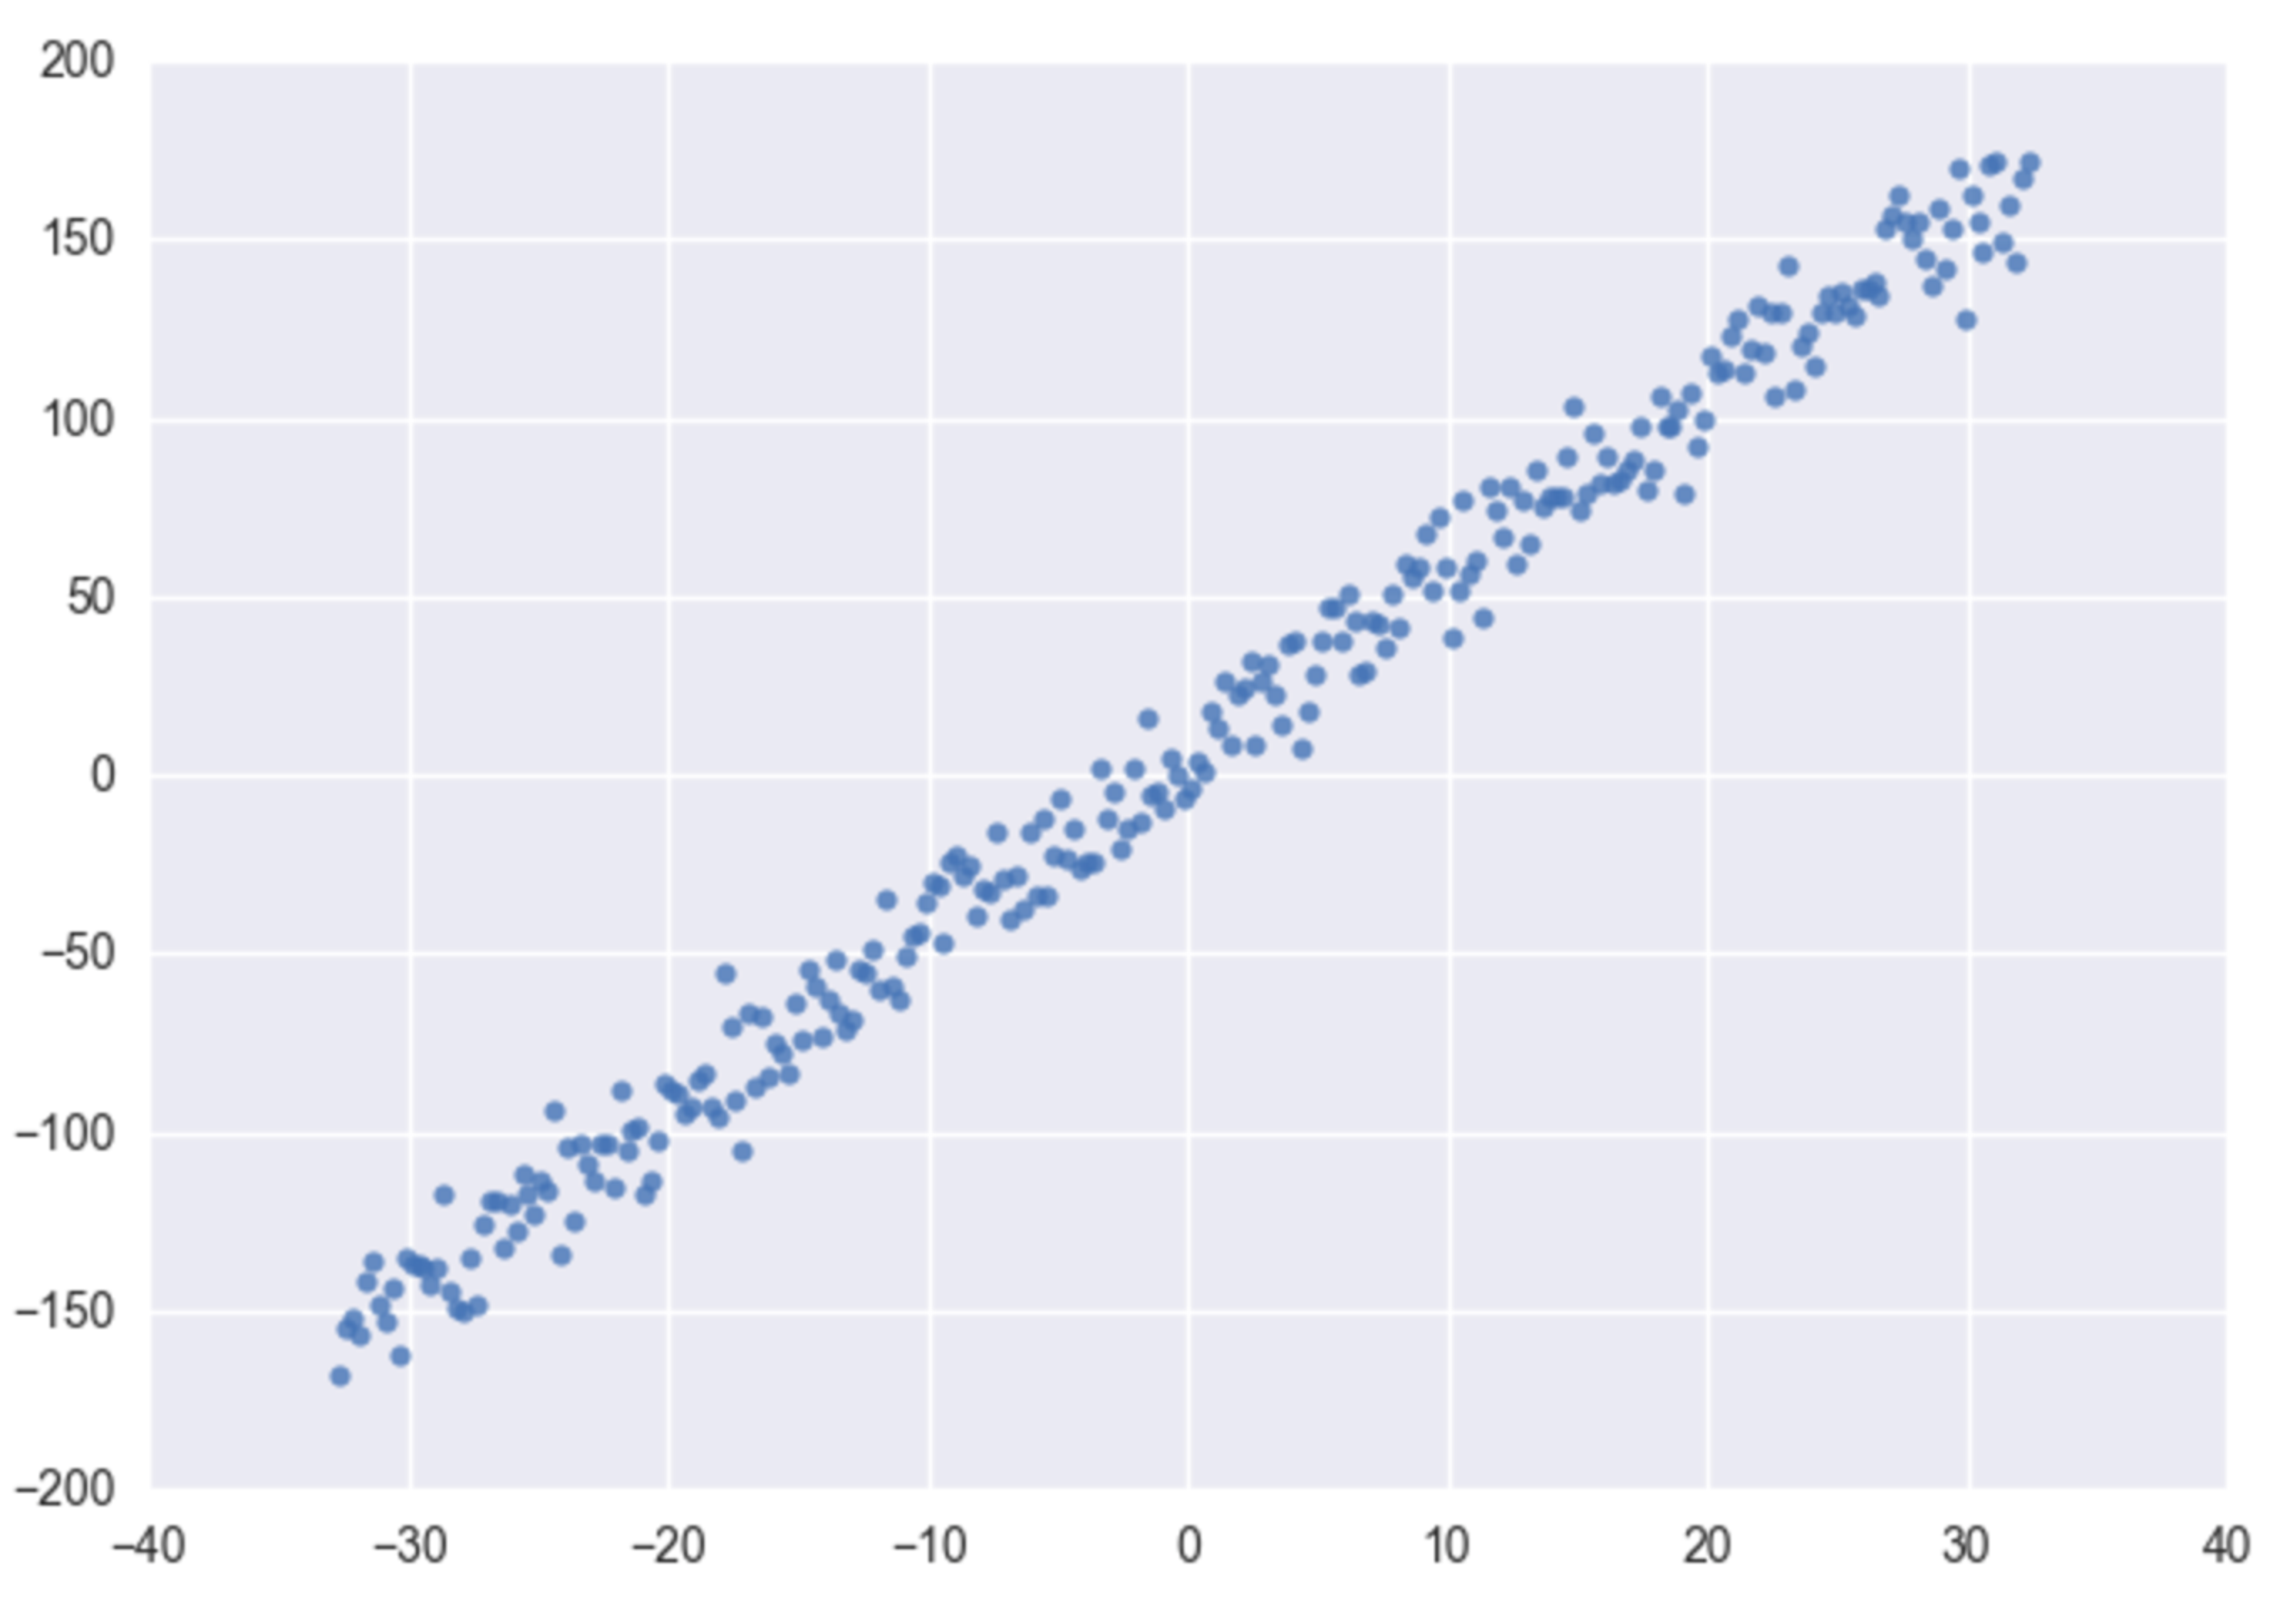
\includegraphics[width=10.0cm]{mh-data.pdf}
\caption{Data}
\end{figure}

\subsubsection{Define Likelihood}
\begin{lstlisting}
def likelihood(param):
    a = param[0][0]
    b = param[0][1]
    sd = param[0][2]
    
    pred = a*x + b # model
    sumSqError = np.power((y - pred), 2).sum()
    
    likelihoodsum = ((sample_size/2)*(np.log(1)-np.log(np.power(sd,2)))) + (- 1/(2*np.power(sd,2)) * sumSqError)
    
    return likelihoodsum
\end{lstlisting}
An error term in the linear regression follows normal distribution. Recall that the normal distribution is $$P(x) = \frac{1}{{\sigma \sqrt {2\pi } }} \exp\left\{  {{{ - \left( {x - \mu } \right)^2 } \mathord{\left/ {\vphantom {{ - \left( {x - \mu } \right)^2 } {2\sigma ^2 }}} \right. \kern-\nulldelimiterspace} {2\sigma ^2 }}}  \right\},$$ and in the linear regression model, mean is given as $\mathbf{x}_i^T \boldsymbol{\beta}$. 
\begin{align}
  \mathcal{L}(\mathbf{y}|\boldsymbol{\beta}, \sigma^2) &= \prod_{i=1}^{n} \frac{1}{(2 \pi \sigma^2)^{\frac{1}{2}}} \exp \left( - \frac{\varepsilon_i^2}{2 \sigma^2}  \right) \\[10pt]
                                                       &= \prod_{i=1}^{n} \frac{1}{(2 \pi \sigma^2)^{\frac{1}{2}}} \exp \left( - \frac{(y_i - \mathbf{x}_i^T \boldsymbol{\beta})^2}{2 \sigma^2}  \right) \\[10pt]
 &= \frac{1}{(2 \pi \sigma^2)^{\frac{n}{2}}} \prod_{i=1}^{n}  \exp \left( - \frac{(y_i - \mathbf{x}_i^T \boldsymbol{\beta})^2}{2 \sigma^2}  \right) \\[10pt]
                                                       &\propto \left( \frac{1}{\sigma^2} \right)^{\frac{n}{2}} \exp \left( - \frac{\sum_{i=1}^{n} (y_i - \mathbf{x}_i^T \boldsymbol{\beta})^2 }{2 \sigma^2} \right)
\end{align}

\subsubsection{Propose parameters}
\begin{lstlisting}[caption={Draw a parameter one by one}]
def next_param(param, param_index):
    a_next = param[0][0] ; b_next = param[0][1] ; sd_next = param[0][2]
    
    if param_index == 0:
        a_next = param[0][0] + npr.normal(0, 0.1)
    elif param_index == 1:
        b_next = param[0][1] + npr.normal(0, 0.1)
    elif param_index == 2:
        sd_next = param[0][2] + npr.normal(0, 0.1)
        
    return np.array([[a_next, b_next, sd_next]])
\end{lstlisting}

\begin{lstlisting}[caption={Draw all parameters at the same tine}]
def next_param2(param):
    a_next = param[0][0] ; b_next = param[0][1] ; sd_next = param[0][2]


    a_next = param[0][0] + npr.normal(0, 0.1)
    b_next = param[0][1] + npr.normal(0, 0.1)
    sd_next = param[0][2] + npr.normal(0, 0.1)

    return np.array([[a_next, b_next, sd_next]])
\end{lstlisting}

\subsubsection{MCMC}
\begin{lstlisting}[caption={Component-wise Sampling}]
num_sampling = 950
chain = np.zeros((num_sampling, 1, 3))
chain[0][0][0] = 20 # starting value for a
chain[0][0][1] = 15 # starting value for b
chain[0][0][2] = 15 # starting value for sd

num_accepted = 0
for i in range(num_sampling-1):
    chain_previous = chain[i][:]
    
    proposal = next_param2(chain[i])

    probab = likelihood(proposal) - likelihood(chain_previous)
    if np.exp(0) < probab: # compare with log likelihood
                           # if it is 0, it converges to MLE
        chain[i+1] = proposal
        num_accepted += 1
    else:
        chain[i+1] = chain[i]
\end{lstlisting}

\begin{lstlisting}[caption={Block-wise Sampling}]
num_sampling = 950
chain = np.zeros((num_sampling, 1, 3))
chain[0][0][0] = 20 # starting value for a
chain[0][0][1] = 15 # starting value for b
chain[0][0][2] = 15 # starting value for sd

num_accepted = 0
for i in range(num_sampling-1):
    chain_previous = chain[i][:]
    chain_new = np.zeros((1, 1, 3))
    
    for p in range(3):
        proposal = next_param(chain_previous, p)
        
        probab = likelihood(proposal) - likelihood(chain_previous)
        if np.exp(0) < probab:
            chain_new[0][0][p] = proposal[0][p]
            num_accepted += 1
        else:
            chain_new[0][0][p] = chain[i][0][p]
            
    chain[i+1] = chain_new[0][:]
\end{lstlisting}

\subsubsection{Results}
\begin{table}[H]
\centering
\caption{Results}
\label{my-label}
\begin{tabular}{|c|c|c|}
\hline
   & MCMC  & True \\ \hline
a  & 5.020 & 5.0  \\ \hline
b  & 6.556 & 7.0  \\ \hline
sd & 9.980 & 10.0 \\ \hline
\end{tabular}
\end{table}

\subsection{Example 2: Multivariate Normal}
Almost same as linear model.

\subsubsection{Create Data Set}
\begin{lstlisting}
y1 = 2 ; y2=5 ; c1=1; c2=10
data = np.random.multivariate_normal(mean=[y1,y2], cov=[[c1, 0], [0, c2]], size=300)
sns.regplot(x=data[: , 0], y=data[: , 1], fit_reg=False)
\end{lstlisting}

\subsubsection{Define Likelihood}
Check the formula on Wikipedia.
\begin{lstlisting}
def likelihood(param): 
    def calc_loglikelihood(residual):
        return -0.5 * (np.log(np.linalg.det(cov1)) + residual.T.dot(np.linalg.inv(cov1)).dot(residual) + 2 * np.log(2 * np.pi))
    
    # mean = np.array([y1, y2]), cov = np.array([[c1, 0], [0, c2]])
    mean1 = np.array([param[0][0], param[0][1]])
    cov1 = np.array([[param[0][2], 0], [0, param[0][3]]])
    residuals = (data - mean1)


    loglikelihood = np.apply_along_axis(calc_loglikelihood, 1, residuals)
    loglikelihoodsum = loglikelihood.sum()

    return loglikelihoodsum
\end{lstlisting}

\subsubsection{Results}
\begin{table}[H]
\centering
\caption{Results}
\label{my-label}
\begin{tabular}{|c|c|c|}
\hline
   & MCMC  & True \\ \hline
y1  & 2.041 & 2.0  \\ \hline
y2  & 5.122 & 5.0  \\ \hline
c1 & 0.9677 & 1.0 \\ \hline
c2 & 9.268 & 10.0 \\ \hline
\end{tabular}
\end{table}


\section{Gibbs Sampling}

\subsection{Theory}
Gibbs sampling utilizes the conditional distribution for each variable so that we do not need a proposal distribution or an accept/reject criterion as in Metropolis-Hasting algorithm. There are two main criterion.
\begin{enumerate}
  \item We have an analytic expression for the conditional distribution of each variable in the joint distribution given all other variables in the joint distribution.
  \item We must be able to sample from each conditional distribution.
\end{enumerate}

\subsection{Bivariate Normal Distribution}
Let's derive the conditional distribution of bivariate normal distribution (see クリエイティブなヴログ for the details).\par
Joint distribution of the multivariate normal distribution is
\begin{align}
f_{\boldsymbol X}(\boldsymbol x)=\frac{1}{(\sqrt{2\pi})^n\sqrt{|\boldsymbol\Sigma|}}\exp{\left \{ -\frac{1}{2}(\boldsymbol x-\boldsymbol\mu)^T\boldsymbol\Sigma^{-1}(\boldsymbol x-\boldsymbol\mu) \right \}}
\end{align}
The $(i,j)$th element of $\boldsymbol{\Sigma}$ is the covariance of $X_i$ and $X_j$ (variance if $i=j$). Bivariate normal distribution is $$\boldsymbol X\sim N\left ( \begin{pmatrix} \mu_X\\ \mu_Y \end{pmatrix},\begin{pmatrix} \sigma_X^2 & \sigma_{XY}\\ \sigma_{XY} & \sigma_Y^2 \end{pmatrix} \right ).$$The joint distribution of $(X,Y)$ is $$f_{XY}(x,y)=\frac{1}{2\pi\sqrt{\sigma_X^2 \sigma_Y^2(1-\rho^2)}}\exp{\left \{ -\frac{\sigma_Y^2(x-\mu_X)^2+2\rho\sigma_X\sigma_Y(x-\mu_X)(y-\mu_Y)+\sigma_X^2(y-\mu_Y)}{2\sigma_X^2 \sigma_Y^2(1-\rho^2)} \right \}}.$$ $\rho$ is a correlation coefficient $\sigma_{XY} / (\sigma_X \sigma_Y)$. We derive $Y$ given $X$ under this distribution.\par
  Integrating out $Y$ from $-\infty$ to $\infty$ gives $$f_X(x)=\frac{1}{\sqrt{2\pi\sigma_X^2}}\exp{\left \{ -\frac{(x-\mu_X)^2}{2\sigma_X^2} \right \}},$$ which is $X \sim \mathcal{N}(\mu_X, \sigma_X^2)$. Use this to calculate conditional distribution of $Y$ $$f_{Y|X}(y|x)=\frac{f_{XY}(x,y)}{f_X(x)} \\ =\frac{1}{\sqrt{2\pi\sigma_Y^2(1-\rho^2)}}\exp{\left \{ -\frac{(y-\mu_Y-\rho\sigma_Y(x-\mu_X)/\sigma_X)^2}{2\sigma_Y^2(1-\rho^2)} \right \}}.$$ Hence, conditional distribution of $Y$ given $X$ is $$N\left ( \mu_Y+\rho\sigma_Y\frac{x-\mu_X}{\sigma_X},\ \sigma_Y^2(1-\rho^2) \right ).$$\par
If we use the definition of $\rho$ $$\rho=\frac{\sigma_{XY}}{\sigma_X\sigma_Y},$$ the conditional distribution becomes \begin{equation} \mathcal{N}\left ( \mu_Y+\frac{\sigma_{XY}}{\sigma_X^2}(x-\mu),\ \sigma_Y^2-\left (\frac{\sigma_{XY}}{\sigma_X^2} \right )^2 \right ).\label{Eq:BiNorm}\end{equation}


\subsection{Example}
We suppose the model with mean $$\boldsymbol{\mu} =  \begin{pmatrix} \mu_1 \\ \mu_2 \end{pmatrix}  = \begin{pmatrix} 0 \\ 0 \end{pmatrix}  ,$$ and covariance $$ \boldsymbol{\Sigma} = \begin{pmatrix} 1 & \rho_{12} \\ \rho_{21} & 1 \end{pmatrix} = \begin{pmatrix} 1 & 0.8 \\ 0.8 & 1 \end{pmatrix} .$$
  Under this condition (see equation (\ref{Eq:BiNorm})), 
\begin{align}
  p(x_1 | x_2^{(t-1)}) &= \mathcal{N} \left(\mu_1 + \rho_{21} (x_2^{(t-1)} - \mu_2), \sqrt{1 - \rho^2_{21}} \right)\\[9pt]
  p(x_2 | x_1^{(t)}) &= \mathcal{N} \left(\mu_2 + \rho_{12} (x_1^{(t)} - \mu_1), \sqrt{1 - \rho^2_{12}} \right)
\end{align}

\subsubsection{Create Dataset}
\begin{lstlisting}
mean = 0 ; c=0.8
data = np.random.multivariate_normal(mean=[mean, mean], cov=[[1, c], [c, 1]], size=200)
\end{lstlisting}
\begin{figure}[H]
\centering
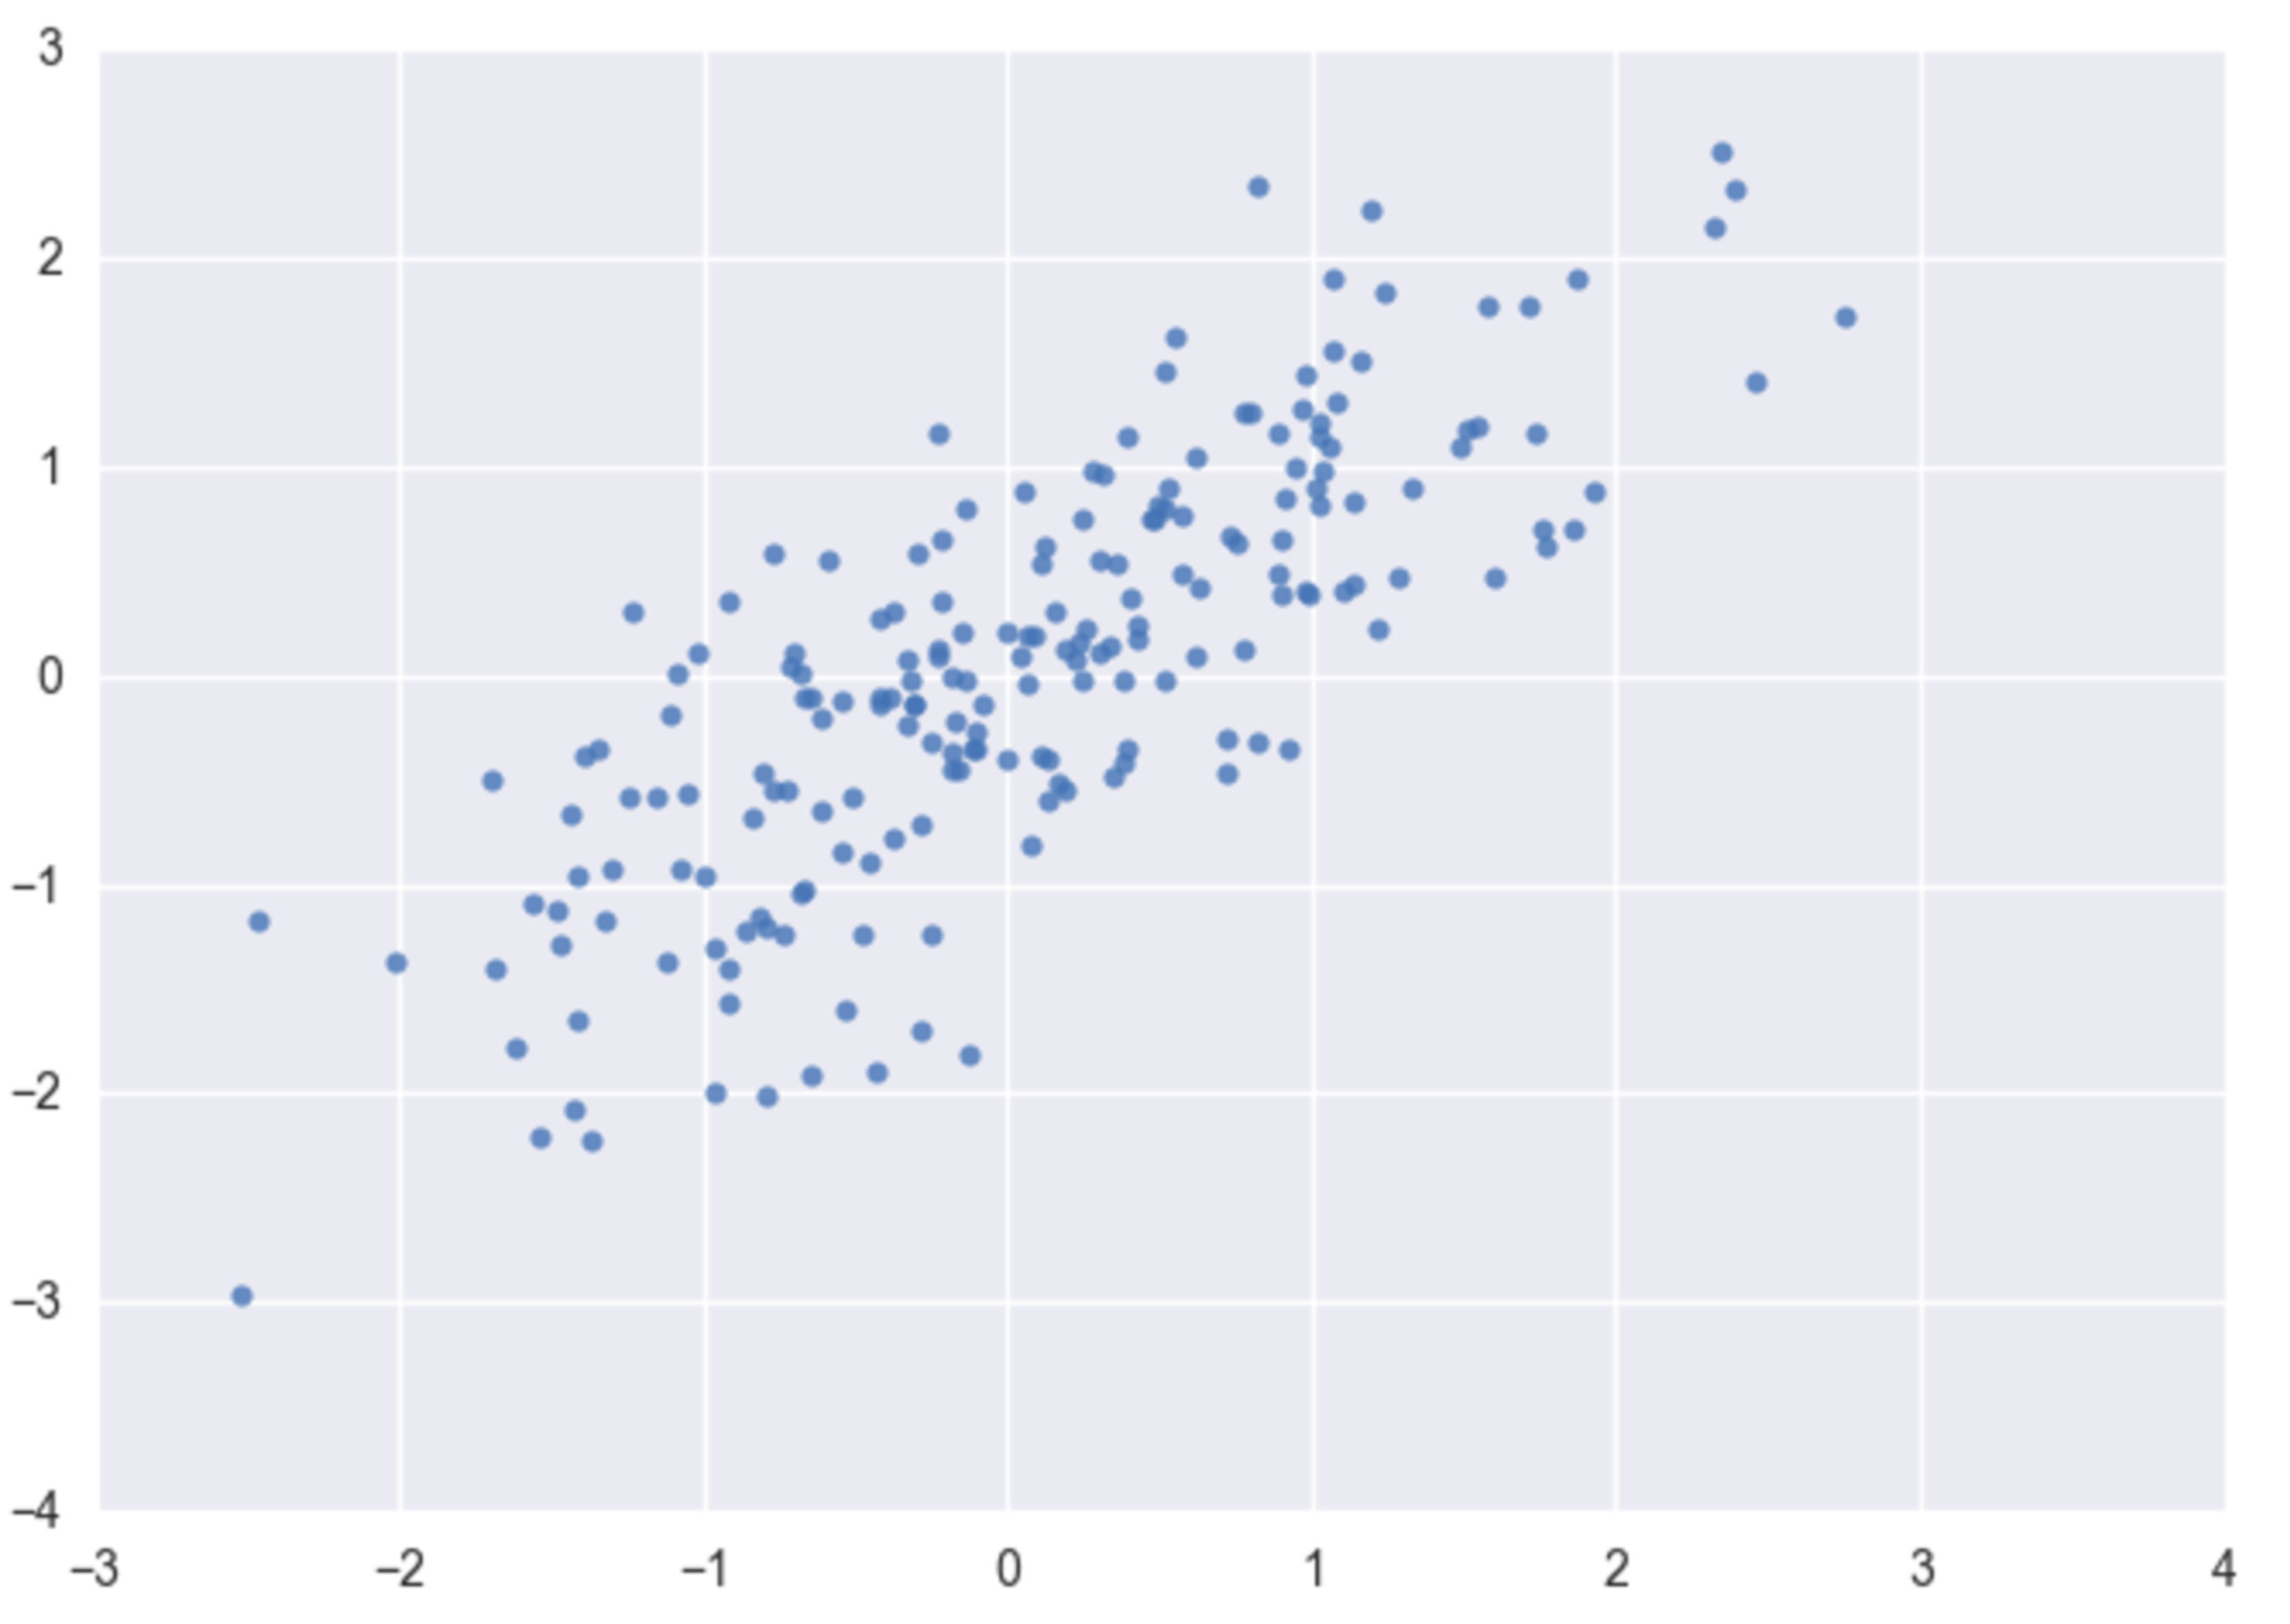
\includegraphics[width=10.0cm]{Gibbs-data.pdf}
\caption{Data}
\end{figure}

\subsubsection{Sampling}
\begin{lstlisting}
num_sampling = 100000
chain = np.zeros((num_sampling, 1, 2))
chain[0][0][0] = npr.uniform(-3,3) # starting value for the first dimension
chain[0][0][1] = npr.uniform(-3,3) # starting value for the second dimension

mu = np.array([data[:, 0].mean(), data[:, 1].mean()])
rho = np.array([np.corrcoef(data[:, 0], data[:, 1])[0,1], np.corrcoef(data[:, 0], data[:, 1])[0,1]])

for i in range(1, num_sampling-1):
    chain_previous = chain[i][:]
    chain_new = np.zeros((1, 1, 2))
    
    muCond = mu[0] + rho[0] * (chain_previous[0][1] - mu[1])
    varCond = np.sqrt( 1 - np.power(rho[0], 2))

    chain_new[0][0][0] = npr.normal(muCond, varCond)
    
    muCond = mu[1] + rho[1] * (chain_new[0][0][0] - mu[0])
    varCond = np.sqrt( 1 - np.power(rho[1], 2))

    chain_new[0][0][1] = npr.normal(muCond, varCond)
            
    chain[i+1] = chain_new[0][:]
\end{lstlisting}

\subsubsection{Results}
\begin{lstlisting}
show_num = int(np.rint(num_sampling * 0.95))
sns.regplot(x=chain[show_num: , 0, 0], y=chain[show_num: , 0, 1], fit_reg=False)
\end{lstlisting}

\begin{figure}[H]
\centering
\includegraphics[width=10.0cm]{Gibbs-result.pdf}
\caption{Gibbs Sampling Result}
\end{figure}

\begin{lstlisting}
> np.cov(chain[show_num: , 0, 0], chain[show_num: , 0, 1])
  array([[ 1.02054775,  0.80871474],
         [ 0.80871474,  1.00932218]])
\end{lstlisting}

\section{Slice Sampling}
\subsection{Theory}
The main idea of slice sampling is to introduce an auxiliary real variable $u$. If the target distribution is $p(z)$, we consider the joint distribution $p(z,u)$. This joint distribution over $z$ and $u$ is over the region $U = \{ (z,u): 0<u<f(z) \}$, and below the curve or surface defined by $f(z)$. The joint density for $(z,u)$ is
\begin{align}
p(z,u) =\begin{cases} 1 / A & {\rm if\ } 0 < u < f(z), \ \ A = \int f(z) dz \\ 0 & {\rm otherwise.} \end{cases} 
\end{align}
The marginal density for $z$ is then,
\begin{align}
  p(z) = \int_{0}^{f(z)} (1/A) du = \frac{f(z)}{A}
\end{align}
To sample for $x$, we can sample jointly for $(z,u)$ and then ignore $u$.\par
Generating independent points uniformly from $U$ is not always easy. One possible solution is to use Gibbs Sampling. We repeat following processes: (1) sample from the conditional distribution for $u$ given $z$, which is uniform over the interval $(0, f(z))$, and (2) sample from the conditional distribution for $z$ given the current $u$, which is uniform over the region $S= \{ z : u < f(z) \}$ and this region $S$ is called ``the slice defined by $u$".

\section*{Reference}
\begin{itemize}
  \item The Clever Machine. MCMC: The Gibbs Sampler. https://theclevermachine.wordpress.com/2012/11/05/mcmc-the-gibbs-sampler/
  \item murawakiの雑記. Slice Sampling for Pruning. https://rekken.g.hatena.ne.jp/murawaki/20131104/p1
  \item 久保拓弥. MCMCからベイズに入ってみる. http://hosho.ees.hokudai.ac.jp/~kubo/stat/2010/Qdai/b/kuboQ2010b.pdf
  \item クリエイティブなヴログ. 二変量正規分布の条件付き分布の解釈. http://kyuuko.s7.valueserver.jp/creation.vsw.jp/bivariate-normal-distribution-328
\end{itemize}

\end{document}
